\section{Physics}
\subsection{Introduction}
Electrokinetic theory describes the dynamics of charged particles
in ionic fluids \cite{kirby2010book}. When a particle acquires surface charge, a layer
of ions of opposite charge is attracted to the surface via
electric forces, creating a double-layer structure around the
particle (see Figure \ref{fig:EDL}). This structure, called
``Debye layer'', electrically screens the surface charge, thus
creating a potential difference between the particle and the outer
layer of the fluid bulk.
\begin{figure}[htbp]
\begin{framed}
    \begin{center}
        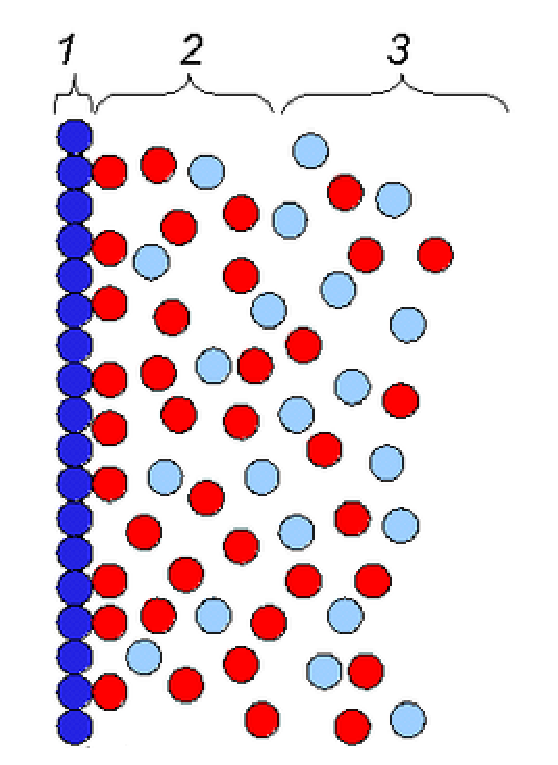
\includegraphics[width=0.25\textwidth]
            {figs/ElectricDoubleLayer.eps}
        \caption{Schematic structure of the double layer:
        (1) particle surface, (2) Debye layer and (3) fluid bulk.
        If the particle surface has positive (blue) surface charge,
        it attracts negative (red) ions from the fluid making the
        Debye layer negatively charged (as opposed to the rest of
        the fluid bulk, which is electrically neutral).
        Zeta potential is defined as the voltage drop on (2).}
        \label{fig:EDL}
    \end{center}
\end{framed}
\end{figure}
In cases where the layer width is much smaller than the particle's
size, an analytical asymptotic solution for the Debye layer
dynamics can be found \cite{yariv2010asymptotic}.

The partial differential equations that descibe the system dynamics
are coupled and non-linear. 
In general, they have no analytic solution. Moreover,
any numerical solver must handle the scale disparity caused by the
Debye layer width being much smaller than the particle's size. A
closed-form linear asymptotic solution has been developed for
spherical ion-exchanging particles and weak electric field in an
axisymmetric setting \cite{yariv2010migration} but it is hard to extend this
analytic solution to more general systems. Once the electric field
becomes stronger, significant nonlinear phenomena are expected.
This interesting regime has not yet been explored.

Recently, it has been conceived that such type of dynamics
can be very useful in transporting and manipulating micro-
and nanoscale objects for many nanotechnology applications,
such as the self-assembly of superstructures, roving sensors, 
drug-delivery systems and useful nanomachinery 
\cite{pumera2010electrochemically,paxton2004catalytic,howse2007self}.
However, since the analytic model for these electrokinetic
phenomena has no closed-form analytic solution, a numerical
solver has to be developed.



%%%%%%%%%%%%%%%%%%%%%%%%%%%%%%%%%%%%%%%%%%%%%%%%%%%%%%%%%%%%%%%%%%%%%%%%%%%%%%%%%%%%%%%%%%%%%%%%%%
\subsection{Micro-scale phenomena}

\subsubsection{Dimensionless Notation}
Positive and negative ionic concentrations are denoted by $c_+$ and $c_-$ respectively.

The respective ionic fluxes are denoted by $\bj_+$ and $\bj_-$.

The electrostatic potential is denoted by $\varphi$. 

The fluid velocity and the pressure field are denoted by $\bv$ and $p$ respectively.

\subsubsection{Nernst-Planck Equations}
The ionic fluxes are given by ions' diffusion, electrostatic forces and ions' advection by the fluid:
\begin{eqnarray}
  \bj_\pm &=& -\bnabla c_\pm \mp c_\pm \bnabla \varphi + \alpha \bv c_\pm
\end{eqnarray}
Due to conservation of ions, the fluxes are divergence-free:
\begin{eqnarray}
\bnabla \cdot \bj_\pm &=& 0.
\end{eqnarray}
These equation may be re-written by using the following transform:
\begin{eqnarray}
  c &=& \frac{c_+ + c_-}{2}\\
  q &=& \frac{c_+ - c_-}{2}
\end{eqnarray}
Thus, salt and charge fluxes are defined by:
\begin{eqnarray}
  \bj &=& \frac{\bj_+ + \bj_-}{2} = -\bnabla c - q \bnabla \varphi + \alpha \bv c \\
  \bi &=& \frac{\bj_+ - \bj_-}{2} = -\bnabla q - c \bnabla \varphi + \alpha \bv q
\end{eqnarray}
And are divergence-free as well:
\begin{eqnarray}
\bnabla \cdot \bj &=& 0 \\
\bnabla \cdot \bi &=& 0 
\end{eqnarray}

\subsubsection{Incompressible Stokes Flow with Electrostatic Force}
Mass conservation (due to constant fluid density):
\begin{eqnarray}
\bnabla \cdot \bv &=& 0
\end{eqnarray}
Momentum conservation (force balance):
\begin{eqnarray}
\Laplacian \bv - \bnabla p + \bnabla \varphi \Laplacian \varphi &=& 0
\end{eqnarray}
Free charge density is given by Poisson equation:
\begin{eqnarray}
\delta^2 \Laplacian \varphi &=& -q
\end{eqnarray}

\subsubsection{Boundary conditions}
Away of the particle, we have uniform flow, uniform electrostatic field
and uniform ionic concentrations:
\begin{eqnarray}
\bv &\rightarrow& -\cU \ui \\
\bE = -\bnabla \varphi &\rightarrow& \beta\ui \\
c_\pm &\rightarrow& 1
\end{eqnarray}

We consider a spherical ion-exchanger. 
At its surface $\mathcal{S}$ (defined at $r=1$ with normal $\bn = \brhat$), 
we have zero slip, anion impermeability, cation selectivity 
and particle's conductance:
\begin{eqnarray}
\bv & = & \bzero \\
\bn \cdot \bj_- & = & 0 \\
c_+ & = & \gamma \\
\varphi & = & \cV
\end{eqnarray}

%%%%%%%%%%%%%%%%%%%%%%%%%%%%%%%%%%%%%%%%%%%%%%%%%%%%%%%%%%%%%%%%%%%%%%%%%%%%%%%%%%%%%%%%%%%%%%%%%%
\subsection{Separation of scales}
When $\delta \ll 1$, 
most of the fluid remains electroneutral ($c_+ \approx c_-$), 
except of a thin boundary layer of width $O(\delta)$, 
also known as ``Debye layer'', around the ion exchanger. 

\subsubsection  {Bulk-scale equations}
Nernst-Planck equations above for the fluid bulk (outside
the boundary layer) using bulk variables:
\begin{eqnarray}
  Q & = & 0 \\
  C & = & C_+ = C_- \\
\bJ &=& -\bnabla C + \alpha \bV C \\
\bI &=& -C \bnabla \varPhi
\end{eqnarray}
Since the flow is incompressible ($\bnabla \cdot V = 0$), 
ion conservation results in the following equations.

\begin{enumerate}
\item Salt conservation macroscale equation:
\begin{eqnarray}
\bnabla \cdot \bJ = \Laplacian C - \alpha \bV \cdot \bnabla C = 0 
\end{eqnarray}

\item Charge conservation macroscale equation:
\begin{eqnarray}
\bnabla \cdot \bI = \bnabla \cdot \pars{ C \bnabla \varPhi } = 0
\end{eqnarray}
\end{enumerate}

Stokes flow equations have the same form:
\begin{eqnarray}
\bnabla \cdot \bV &=& 0 \\
\Laplacian \bV - \bnabla P + \bnabla \varPhi \Laplacian \varPhi &=& 0
\end{eqnarray}

\subsubsection{Debye-scale effective boundary conditions}
We define the rescaled coordinate $\rho$ (normal to ion-exchanger surface), where $\delta \ll 1$:
\begin{eqnarray}
  \rho &=& \frac{r-1}{\delta} 
\end{eqnarray}
Thus, the electric potential and the ionic concentrations are $O(1)$ at Debye layer ($r \approx 1$):
\begin{eqnarray}
  \varphi(\rho,\theta) &\sim& \varphi \\
  c_\pm(\rho,\theta) &\sim& c_\pm \\
  c(\rho,\theta) &\sim& c \\
  q(\rho,\theta) &\sim& q
\end{eqnarray}

The radial fluxes at the Debye layer are $O(\delta^{-1})$, due to coordinate rescaling:
\begin{eqnarray}
  j_\pm(\rho, \theta) &\sim& \delta^{-1} j_\pm
\end{eqnarray}

The pressure is $O(\delta^{-2})$, due to momentum balance equations:
\begin{eqnarray}
  p(\rho, \theta) &\sim& \delta^{-2} p
\end{eqnarray}

The tangential velocity component is $O(1)$ and the radial one is $O(\delta)$.

In order to match bulk $O(1)$ outer radial ionic flux, 
the $O(\delta^{-1})$ term of the inner ionic radial flux $j_\pm(\rho, \theta)$ must vanish:
\begin{eqnarray}
  -\deriv{c_\pm}{\rho} \mp c_\pm \deriv{\varphi}{\rho} &=& 0 \\
  \deriv{\varphi}{\rho} \pm\frac{1}{c_\pm}\deriv{c_\pm}{\rho} &=& 0 \\
  \pars{\varPhi - \varphi} \pm\pars{\log C_\pm - \log c_\pm} &=& 0 \\
  \varPhi - \varphi \pm \log \frac{C_\pm}{c_\pm} &=& 0
\end{eqnarray}
This relation can be rewritten as Boltzmann distribution of ionic concentration:
\begin{eqnarray}
\lim_{\rho\rightarrow\infty} c_\pm &=& C \\
c_\pm &=& C \exp\left[\pm(\varPhi - \varphi)\right]
\end{eqnarray}

Due to cation selectivity, $c_+|_{\rho=0} = \gamma$.
\begin{eqnarray}
  c_+ = \gamma &=& C \exp(\varPhi - \cV) \\
  \cV + \log \gamma &=& \log C + \varPhi
\end{eqnarray}

Denote zeta potential as the voltage drop between the particle surface and the end of
the boundary layer, $\zeta = \cV - \varPhi$. 

Without loss of generality, 
we assume that $\cV = -\log\gamma$, thus $\zeta = -\log\gamma-\varPhi$:
\begin{eqnarray}
\varPhi + \log C &=& 0
\end{eqnarray}

Due to anion impermeability and radial flux continuity:
\begin{eqnarray}
  \br \cdot \bj_- = -\deriv{c_-}{r} + c_- \deriv{\varPhi}{r} &=& 0 \\
-\deriv{C}{r} + C \deriv{\varPhi}{r} &=& 0 \\
\deriv{}{r}\pars{\varPhi - \log C} &=& 0
\end{eqnarray}

Using the derivation at Appendix \ref{append:slip} and that $V_r = 0$ 
on the boundary, the slip condition can be written using surface
gradient operator:
\begin{eqnarray}
\bV &=& 
\zeta \cdot \bnabla_\mathcal{S} \varPhi 
+ 2\log\pars{1-\tanh^2\frac{\zeta}{4}} \cdot \bnabla_\mathcal{S} \log C \\
\bnabla_\mathcal{S} &=& \pars{\tI - \bn\bn} \bnabla
\end{eqnarray}

\subsection{Steady state}
The stress tensor is composed of Newtonian and Maxwel stresses:
\begin{eqnarray}
\tT &=& \bnabla \bV + (\bnabla \bV)^\dagger - P \tI
+ \bnabla \varPhi \bnabla \varPhi - \frac{1}{2} (\bnabla \varPhi \cdot \bnabla \varPhi) \tI \\
\bnabla \cdot \tT &=& \bzero
\end{eqnarray}
The total force acting on the particle is computed by the following surface integral:
\begin{eqnarray}
\bF &=& \oint_\mathcal{S} \tT \cdot \bnhat  dA 
\end{eqnarray}
In steady state (constant particle drift velocity $\cU$), it should be zero: 
\begin{eqnarray}
\bF = \bzero
\end{eqnarray}
